% -------------------------------------------------------------------------------
% Establish page structure & font.
\documentclass[12pt]{report}

\usepackage[total={6.5in, 9in},
	left=1in,
	right=1in,
	top=1in,
	bottom=1in,]{geometry} % Page structure

\usepackage{graphicx} % Required for inserting images
\graphicspath{{../.images/}} % Any additional images I use (BCU logo, etc) are from here.

\usepackage[utf8]{inputenc} % UTF-8 encoding
\usepackage[T1]{fontenc} % T1 font
\usepackage{float}  % Allows for floats to be positioned using [H], which correctly
                    % positions them relative to their location within my LaTeX code.
\usepackage{subcaption}
% \usepackage[british]{babel}
\usepackage{csquotes}

\usepackage{pdflscape} % Enables the page to be rotated 
                       % landscape for easier image viewing.

% -------------------------------------------------------------------------------
% Declare biblatex with custom Harvard BCU styling for referencing.
\usepackage[
    useprefix=true,
    maxcitenames=2,
    maxbibnames=99,
    style=authoryear,
    dashed=false, 
    natbib=true,
    url=false,
    backend=biber
]{biblatex}

% Additional styling options to ensure Harvard referencing format.
\renewbibmacro*{volume+number+eid}{
    \printfield{volume}
    \setunit*{\addnbspace}
    \printfield{number}
    \setunit{\addcomma\space}
    \printfield{eid}}
\DeclareFieldFormat[article]{number}{\mkbibparens{#1}}

% Declare it as the bibliography source, to be called later via \printbibliography
\addbibresource{litReview.bib}

% -------------------------------------------------------------------------------
% To prevent "Chapter N" display for each chapter
\usepackage[compact]{titlesec}
\usepackage{wasysym}
\usepackage{import}

\titlespacing*{\chapter}{0pt}{-2cm}{0.5cm}
\titleformat{\chapter}[display]
{\normalfont\bfseries}{}{0pt}{\Huge}

% -------------------------------------------------------------------------------
% Custom macro to make an un-numbered footnote.

\newcommand\blfootnote[1]{
    \begingroup
    \renewcommand\thefootnote{}\footnote{#1}
    \addtocounter{footnote}{-1}
    \endgroup
}

% -------------------------------------------------------------------------------
% Fancy headers; used to show my name, BCU logo and current chapter for the page.
\usepackage{fancyhdr}
\usepackage{calc}
\pagestyle{fancy}

\setlength\headheight{37pt} % Set custom header height to fit the image.

\renewcommand{\chaptermark}[1]{%
    \markboth{#1}{}} % Include chapter name.


% Lewis Higgins - ID 22133848           [BCU LOGO]                [CHAPTER NAME]
\lhead{Lewis Higgins - ID 22133848~~~~~~~~~~~~~~~
\includegraphics[width=1.75cm]{BCU}}
\fancyhead[R]{\leftmark}

% ------------------------------------------------------------------------------
% Used to add PDF hyperlinks for figures and the contents page.

\usepackage{hyperref}

\hypersetup{
    colorlinks=true,
    linkcolor=black,
    filecolor=magenta,
    urlcolor=blue,
    citecolor=black,
}

% ------------------------------------------------------------------------------
\usepackage{xcolor} 
\usepackage{colortbl}
\usepackage{longtable}
\usepackage{amssymb}
% ------------------------------------------------------------------------------

% ------------------REMOVE ME --------------------------------------------------

% Temp, using to add notes for the draft edition.
\usepackage{tcolorbox}

% ----------------- REMOVE ME --------------------------------------------------

\begin{document}

    \makeatletter
    \begin{titlepage}
        
\includegraphics[width=0.3\linewidth]{BCUWide.jpg}\\[4ex]
        \vspace{1cm}
        \begin{center}
            {\huge \bfseries  CMP6200}\\[2ex]
            {\huge \bfseries  Individual Undergraduate Project}\\[2ex]
            {\huge \bfseries 2024 - 2025}\\[6ex]
            {\large \bfseries A2 - Literature Review and Methods}\\[10ex]
            {\huge \bfseries University Artificially Intelligent Assistant}\\[6ex]
            
\includegraphics[width=0.1\linewidth]{Symbol.png}\\[40ex]
            Course: Computer \& Data Science\\
            Student Name: Lewis Higgins\\
            Student Number: 22133848\\
            Supervisor Name: Dr. Atif Azad
        \end{center}
    \end{titlepage}
    \makeatother
    \thispagestyle{empty}
    \newpage

    \tableofcontents
    %\footnotesize{\listoffigures}

    \chapter{Report Introduction}\label{ch:introduction}
    \section{Aims and Objectives}

    \noindent
    This project aims to aid new and existing students alike while they are attending university with 
    helpful information about university itself, such as university societies, locations/campuses, 
    and policies through the medium of a digital chatbot companion to converse with.
    The project's objectives are:

    \begin{itemize}
        \item Conduct a thorough literature review on the surrounding topics, namely AI, LLMs and NLP.
        \item Create effective documentation for all stages of development, highlighting challenges faced during the process.
        \item Leverage Retrieval-Augmented Generation alongside a cloud-based LLM to query a vector database of university-related data.
        \item Develop a chatbot capable of accurately answering user queries related to university 
        buildings, policies, and societies with a minimum 80\% accuracy rate.
        \item Evaluate the effectiveness of an AI assistant on university student acclimatization.
    \end{itemize}

    \pagebreak % REMOVE ME IF UNNECESSARY

    \section{Literature Search Methodology}

    \noindent 
    My literature search will be performed using multiple reputable databases for academic papers, including:
    \begin{itemize}
        \item IEEE Xplore
        \item Scopus / Elsevier
        \item Google Scholar
        \item arXiv
        \item BCU Online Library
    \end{itemize}
    
    \noindent By using multiple different databases to source my information from, I can ensure that
    any potentially relevant literature will be found. Figure \ref{fig:litSearch} depicts 
    how in a search for articles about employee retention, only 25.7\% appeared in multiple databases
    \autocite{litSearch}, meaning that the remaining 74.3\% of articles were exclusive to the single 
    database in which they were found, emphasising the importance of searching multiple databases.  

    \begin{figure}[H]
        \centering
        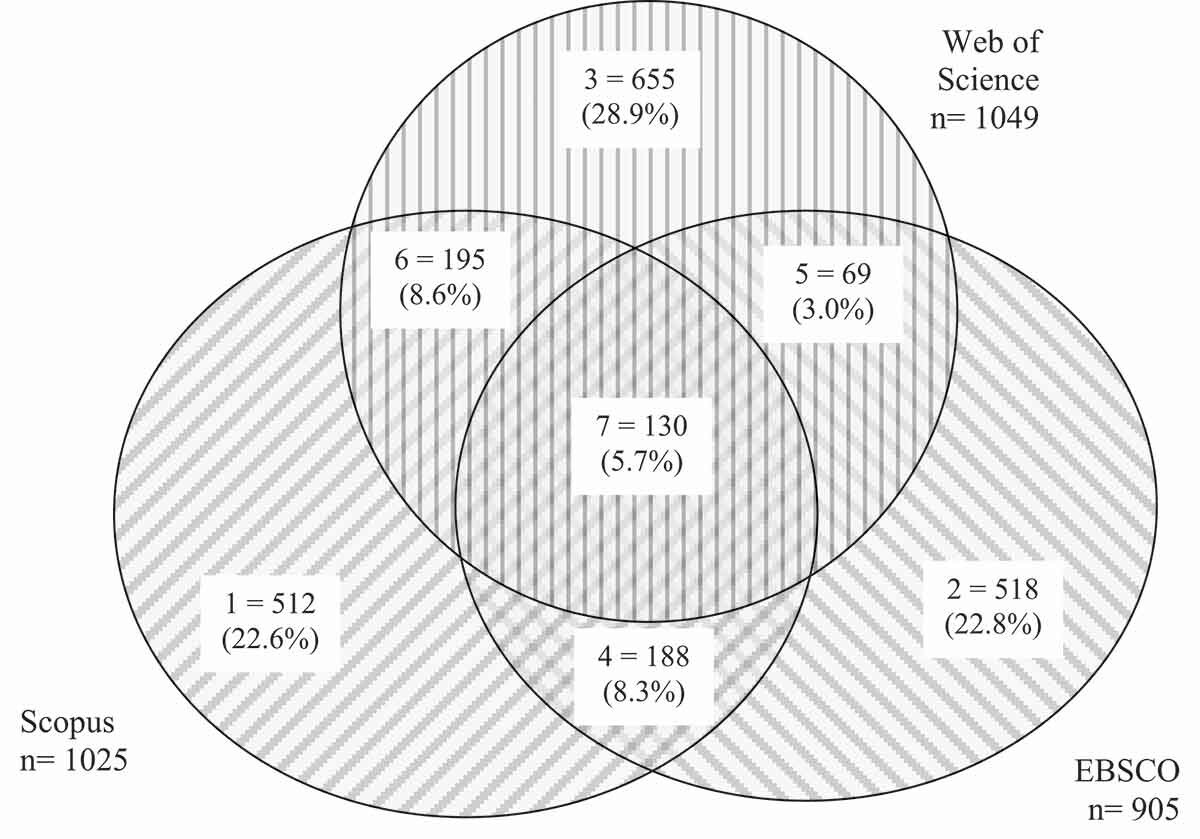
\includegraphics[width=.6\linewidth]{litSearchDBs.jpg}
        \caption{Distribution of searched articles across databases. \autocite{litSearch}}
        \label{fig:litSearch}
    \end{figure}
   
    \noindent 
    All searches performed for recent literature will have a heavy preference 
    to more recent literature, due to the constantly evolving fields my project is based on. 
    The search terms I will use to retrieve the data I will be studying are:

    \begin{itemize}
        \item Artificial Intelligence / AI 
        \item Natural Language Processing / NLP
        \item Large Language Models / LLMs
        \item Chatbots / Conversational Agents
        \item Retrieval-Augmented Generation / RAG
        
        
        % =========================================================
        % To be removed?
        % \item User Experience / UX
        % \begin{itemize}
        %     \item Human-Computer Interaction
        % \end{itemize}
        % =========================================================
    \end{itemize}

    \noindent
    By using these specific terms that are directly relevant to the core themes of my project,
    I will be ensuring that I only retrieve literature that will be of crucial use in its 
    development.


    \chapter{Literature Review}

    \section{Themes}

    To develop the artefact and conduct thorough background research on relevant literature to further my 
    knowledge of the subject areas, key general themes of the project were identified in Table \ref{tab:themes}. From these themes, further 
    keywords to be used in the literature search were derived to ensure that retrieved literature is directly relevant 
    to my research and development of the final artefact. Due to the constantly evolving fields the project focuses 
    on, it will be necessary to limit the results to primarily those written in recent years as there are 
    frequent new developments in the subject areas.

    % \begin{tcolorbox}[colback=red!5!white,colframe=red!75!black,title=Significant uncertainty]
    %     I had a large amount of difficulty identifying my project's key themes, as many of them overlap and I was
    %     unsure which would simply be keywords of others, which is most evident with "AI" and "Generative AI" seen below.
    %     From what I can gather so far, I'm not sure if just making a chatbot that just accesses another LLM's API is worthy 
    %     of being a dissertation project at all, and if it would be better to try with my own fine-tuned model of something 
    %     like LLaMA. I'd have much more to write about that way.
    % \end{tcolorbox}
\pagebreak
    \begin{table}[H]
        \centering
        \begin{tabular}{|p{0.2\textwidth}|p{0.55\textwidth} | p{0.2\textwidth}|}
            \hline
            \cellcolor{blue!25}Theme & \cellcolor{blue!25}Description &
            \cellcolor{blue!25}Keywords \\

            \hline

            AI & A field of computing dedicated to allowing computers to simulate human
            learning by training them on large amounts of data so that they can recognise patterns to classify or 
            predict unknown data. AI can only be as good as the data it is trained upon, and can 
            develop biases if it is fed too much data of a certain type. & Generative AI, 
            Human-Centred AI, Explainable AI, AI Ethics, AI Bias \\

            % \hline

            % Generative AI & AI dedicated to the generation of content rather than prediction or 
            % classification. It is possible for generative AI to produce text, images and 
            % more recently, even video and sound. & LLMs, Tokens, Embedding \\

            \hline

            Natural Language Processing & NLP refers to the use of machine learning to encode and 
            process text to understand it in a similar way to humans, which can be used to allow direct 
            two-way conversation between users and computers. & Embedding models, Vectorisation
            Semantic search, Entity linking

            \\

            \hline
            
            LLMs & Large Language Models are a type of machine learning model dedicated to the recognition and generation of text.
            As suggested by their name, they are trained on enormous amounts of text data, which allows them 
            to have active conversations with users. There are many different LLMs, and as their size and 
            complexity increases, so too does the necessary processing power. &
            Fine-tuning, Prompt engineering, Impact on industry,
            GPT4o, LLaMA, Gemini, Evaluation
            
            \\
            \hline 

            Retrieval-Augmented Generation \newline (RAG) & The optimisation of the generated text output of an LLM, incorporating
            an external data source to enhance its contextual knowledge and enhancing the subject relevancy of outputs.
            & Embedding, Vector databases, Document retrieval, Prompt engineering\\

            \hline
            Chatbot \newline Conversational Agent & Software that simulates a natural conversation between the 
            computer and end user. Many chatbots, including the one to be produced in this project, utilise recent
            developments such as Generative AI and natural language processing (NLP) to interpret and respond to user queries.
            \autocite{IBMChatbotDef}
            & NLP, Digital assistant, ChatGPT, Risks, Impact on industry \\

            % \hline

            % User Experience (UX) & The end user's overall experience of using a system, such as its ease of use and 
            % whether it is enjoyable to use \autocite{UXDict}. In the context of this project, it will refer to the user's 
            % ability to smoothly converse with the chatbot and how human-like it is. 
            % & Conversational design, usability, accessibility, human-computer interaction

            % \\

            \hline 

        \end{tabular}
        \caption{The themes and keywords used in the literature search.}
        \label{tab:themes}
    \end{table}


    \pagebreak % REMOVE IF NECESSARY

    \section{Review of Literature}

    \subsection{Artificial Intelligence (AI)}

    % Restructure, and likely cut down on the word count if you can? It does seem like this could all be relevant.

    Researchers have always wanted to harness the processing power of computers to act in a similar manner 
    indistinguishable from that of humans from as long ago as 1950, where the question was posed 
    'Can machines think?' \autocite{turing_icomputing_1950}. Ever since, constant innovations were made in computer 
    intelligence and machine learning, from playing games of checkers at a better level than human players \autocite{samuel_studies_1959}
    to classifying the contents of millions of images using convolutional neural networks \autocite{krizhevsky_imagenet_2012}.

    Recently, AI is used across many disciplines for different purposes to complete tasks faster than, and in some cases better than,
    human workers. \textcite{wirtz_brave_2018} write that 'service robots'~\footnote{Defined as "system-based autonomous and adaptable interfaces that 
    interact, communicate and deliver service to an organization’s customers" \autocite[p.909]{wirtz_brave_2018}} can complete a variety of 
    tangible or intangible actions, such as two-way conversation with chatbots.
    
    \begin{figure}[H]
        \centering
        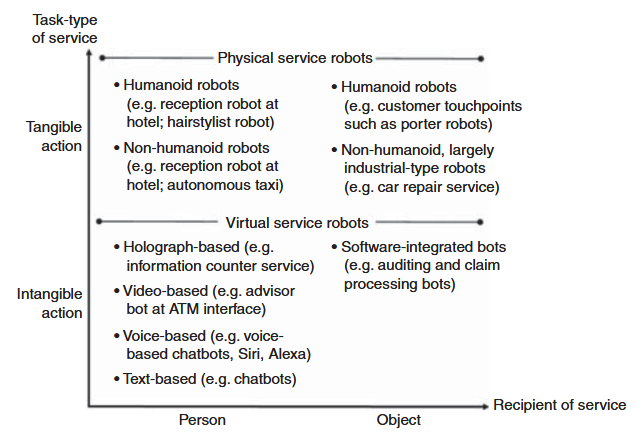
\includegraphics[width=.8\linewidth]{serviceBots.png}
        \caption{Service robots categorization by task-type and recipient of service \autocite{wirtz_brave_2018}.}
        \label{fig:serviceBots}
    \end{figure}

    AI is still a constantly evolving field that is seeing bleeding-edge developments on a 
    highly frequent basis and is becoming instrumental in many people's work and private lives 
    with the introduction of large language models (LLMs) \autocite{AIDigitalAssistants}.


    However, when developing a project that utilises AI, it is important that the development process
    is ethical and human-centred, which is known as Human-Centred AI (HCAI). 
    Another issue is the "black-box problem" - the inability to know an AI's reasoning, meaning that 
    eXplainable AI (XAI) is a growing necessity \autocite{miro-nicolau_comprehensive_2025}. 
    
    In focusing on HCAI and XAI, the focus shifts from the machine executing the algorithms, and instead to the user and their experience 
    using the AI. \textcite{AIEthics} strongly advocates for the 
    promotion of HCAI for the benefit of both companies and their users, which is a commonly accepted 
    idea due to the ethical risks of using AI. 
    
    Because AI calculates outcomes from its training data rather 
    than understanding social norms and perspectives, the use of it in sociotechnical systems poses serious risks 
    due to the 'traps' it can fall into, because it cannot account for every possibility such as the personal tendencies 
    and biases of its users \autocite{selbst_fairness_2019}, and therefore developers require a shift in focus - from the final product
    at the end of development to the development process itself and end users, which also echoes Shneiderman's views. 

    \subsection{Natural language processing (NLP)}
    The ability for a computer to interpret and understand human language greatly enhances the scale of their capabilities. This was 
    recognised during the 1950s, where machine translation from Russian to English was demonstrated for the first time, albeit in a basic form \autocite{zampolli_natural_1994}.
    Ever since, NLP has persistently been a key topic in computing, and even more so become in recent years, with its applications becoming very wide 
    in scope with modern processing power.

    One of the key advancements in NLP is vectorisation, a process where data is embedded into a numerical equivalent that a computer can interpret, 
    enabling Natural Language Understanding (NLU) and the identification of semantic similarities between words through the use of an embedding model 
    like Word2Vec \autocite{mikolov_efficient_2013} without the need to manually label data. 
    Word2Vec was a key innovation in NLP, and Mikolov and Le went on to improve it further with Doc2Vec \autocite{le_distributed_2014}, which could embed 
    entire documents into semantically searchable vectorised forms.
    
    Embedding models have further improved since, most notably with \textcite{vaswani_attention_2017}'s Transformer architecture enhancing models such as 
    BERT \autocite{devlin_bert_2019}, which is able to analyse context through analysing multiple neighbours of a word rather than reading from left to right,
    gaining a higher understanding of the text it processes. Many embedding models have since been developed, though one of the most reputable is OpenAI's 
    recent text-embeddings-3 model \autocite{openai_vector_nodate}, which can be used in the development of the chatbot at a low cost. 
    

    \pagebreak 

    \subsection{Large language models}
    % Restructure, and talk about the evaluation of generated answers!

    LLMs are colossal machine learning models that leverage NLP to generate text, and have become widely used across 
    industries in place of technical support and human resources \autocite{vrontis_artificial_2022}. The training data required for an LLM is immense, 
    reaching 45 terabytes of text data for ChatGPT in 2023 \autocite{dwivedi_so_2023}. 
    
    This data is harvested from websites \autocite{dubey_llama_2024}
    and social media due to it being one of the largest repositories of opinionated text data \autocite{wang_fine-grained_2016}. 
    However, meticulous care is taken into the specific sources used to remove 
    Personally Identifiable Information (PII) to minimise privacy and ethical concerns \autocite{dubey_llama_2024}.
    
    The previously mentioned Transformer from \textcite{vaswani_attention_2017} 
    became a staple in LLMs due to the major reduction in necessary processing power to produce higher-quality 
    results, and it continues to underpin many LLMs today, including ChatGPT \autocite{brown_language_2020}. 
    Even with these enhancements, LLMs are still extremely performance intensive,
    requiring more than 8 top-range server-grade GPUs to run some of the most powerful high-parameter models like LLaMA 3.1's 405 billion parameter model \autocite{dubey_llama_2024},
    and many therefore use cloud API solutions to access LLMs.
    
    The amount of parameters in a model does not entirely account for the quality of its responses, as studied by \textcite{ouyang_training_2022}
    in Figure \ref{fig:LLMPref} wherein their surveys revealed their fine-tuned LLM "InstructGPT" with over 100x less parameters than a 175 billion parameter 
    GPT3 model would often give answers preferred by its human assessors, which reveals that the fine-tuning and prompt engineering of an LLM is as vitally important
    to the quality of its responses as the amount of parameters.  
    
    % Another major innovation in LLMs came in the form of Retrieval-Augmented 
    % Generation (RAG), which allows LLMs to generate answers based on an additional external data source \autocite{lewis_retrieval-augmented_2021}, such as a company's own database.
    % RAG therefore allows pre-trained LLMs to be attached to another data source and generate text based on that source, which can help to reduce 
    % LLM "hallucinations" \autocite{lewis_retrieval-augmented_2021}, which are occurrences where the LLM will fabricate false information as though it were correct, 
    % due to the fact that it can retrieve the relevant information it otherwise may not have had.

    \begin{figure}[H] 
        \centering
        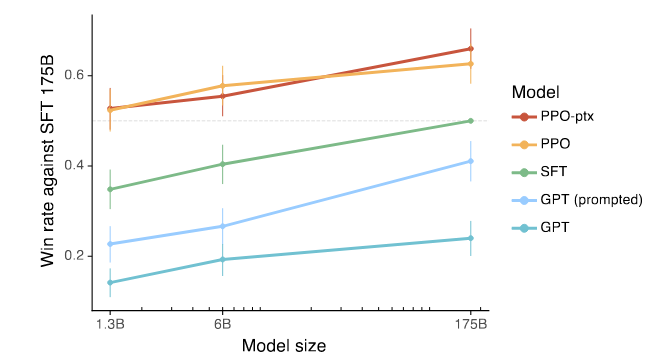
\includegraphics[width=.85\linewidth]{ouyangLLMPreference.png}
        \caption{Human evaluations of the GPT models produced by \textcite{ouyang_training_2022}. PPO and PPO-ptx are their models.}
        \label{fig:LLMPref}
    \end{figure}

    The simplest way to measure the accuracy and quality of an LLM's responses is through human evaluation surveys such as that conducted by \textcite{ouyang_training_2022}, though
    software approaches such as the open-source DeepEval can be used. DeepEval offers 14 metrics to test LLM outputs with \autocite{deepeval_introduction_2024},
    with a notable metric being "G-Eval", originally introduced by \textcite{liu_g-eval_2023}, which uses an "LLM-as-a-judge" approach where an LLM will evaluate
    and grade the quality of the output.


    \subsection{Retrieval-Augmented Generation}
    % Does UX/HCI get axed in favour of this? The AI section is really long and takes up a lot of the word count,
    % so shortening that is also an option.
    
    % Talk about the evaluation of generated answers here maybe?
    While LLMs are highly useful tools across many industries, they are not without limitations. The most notable 
    of these limitations are hallucinations \autocite{lewis_retrieval-augmented_2021}, where the LLM will fabricate 
    information that conflicts with user input, earlier conversation context or true facts \autocite{zhang_sirens_2023}. This occurs as a direct result of the LLM's parametric memory\footnote{Knowledge that the LLM has from its training data \autocite{siriwardhana_improving_2023}.}
    being overfitted or biased, which can be counteracted through introducing an external knowledge source, known as non-parametric memory (\textcite{komeili_internet-augmented_2022}, \textcite{siriwardhana_improving_2023}).
    
    \begin{figure}[H] 
        \centering
        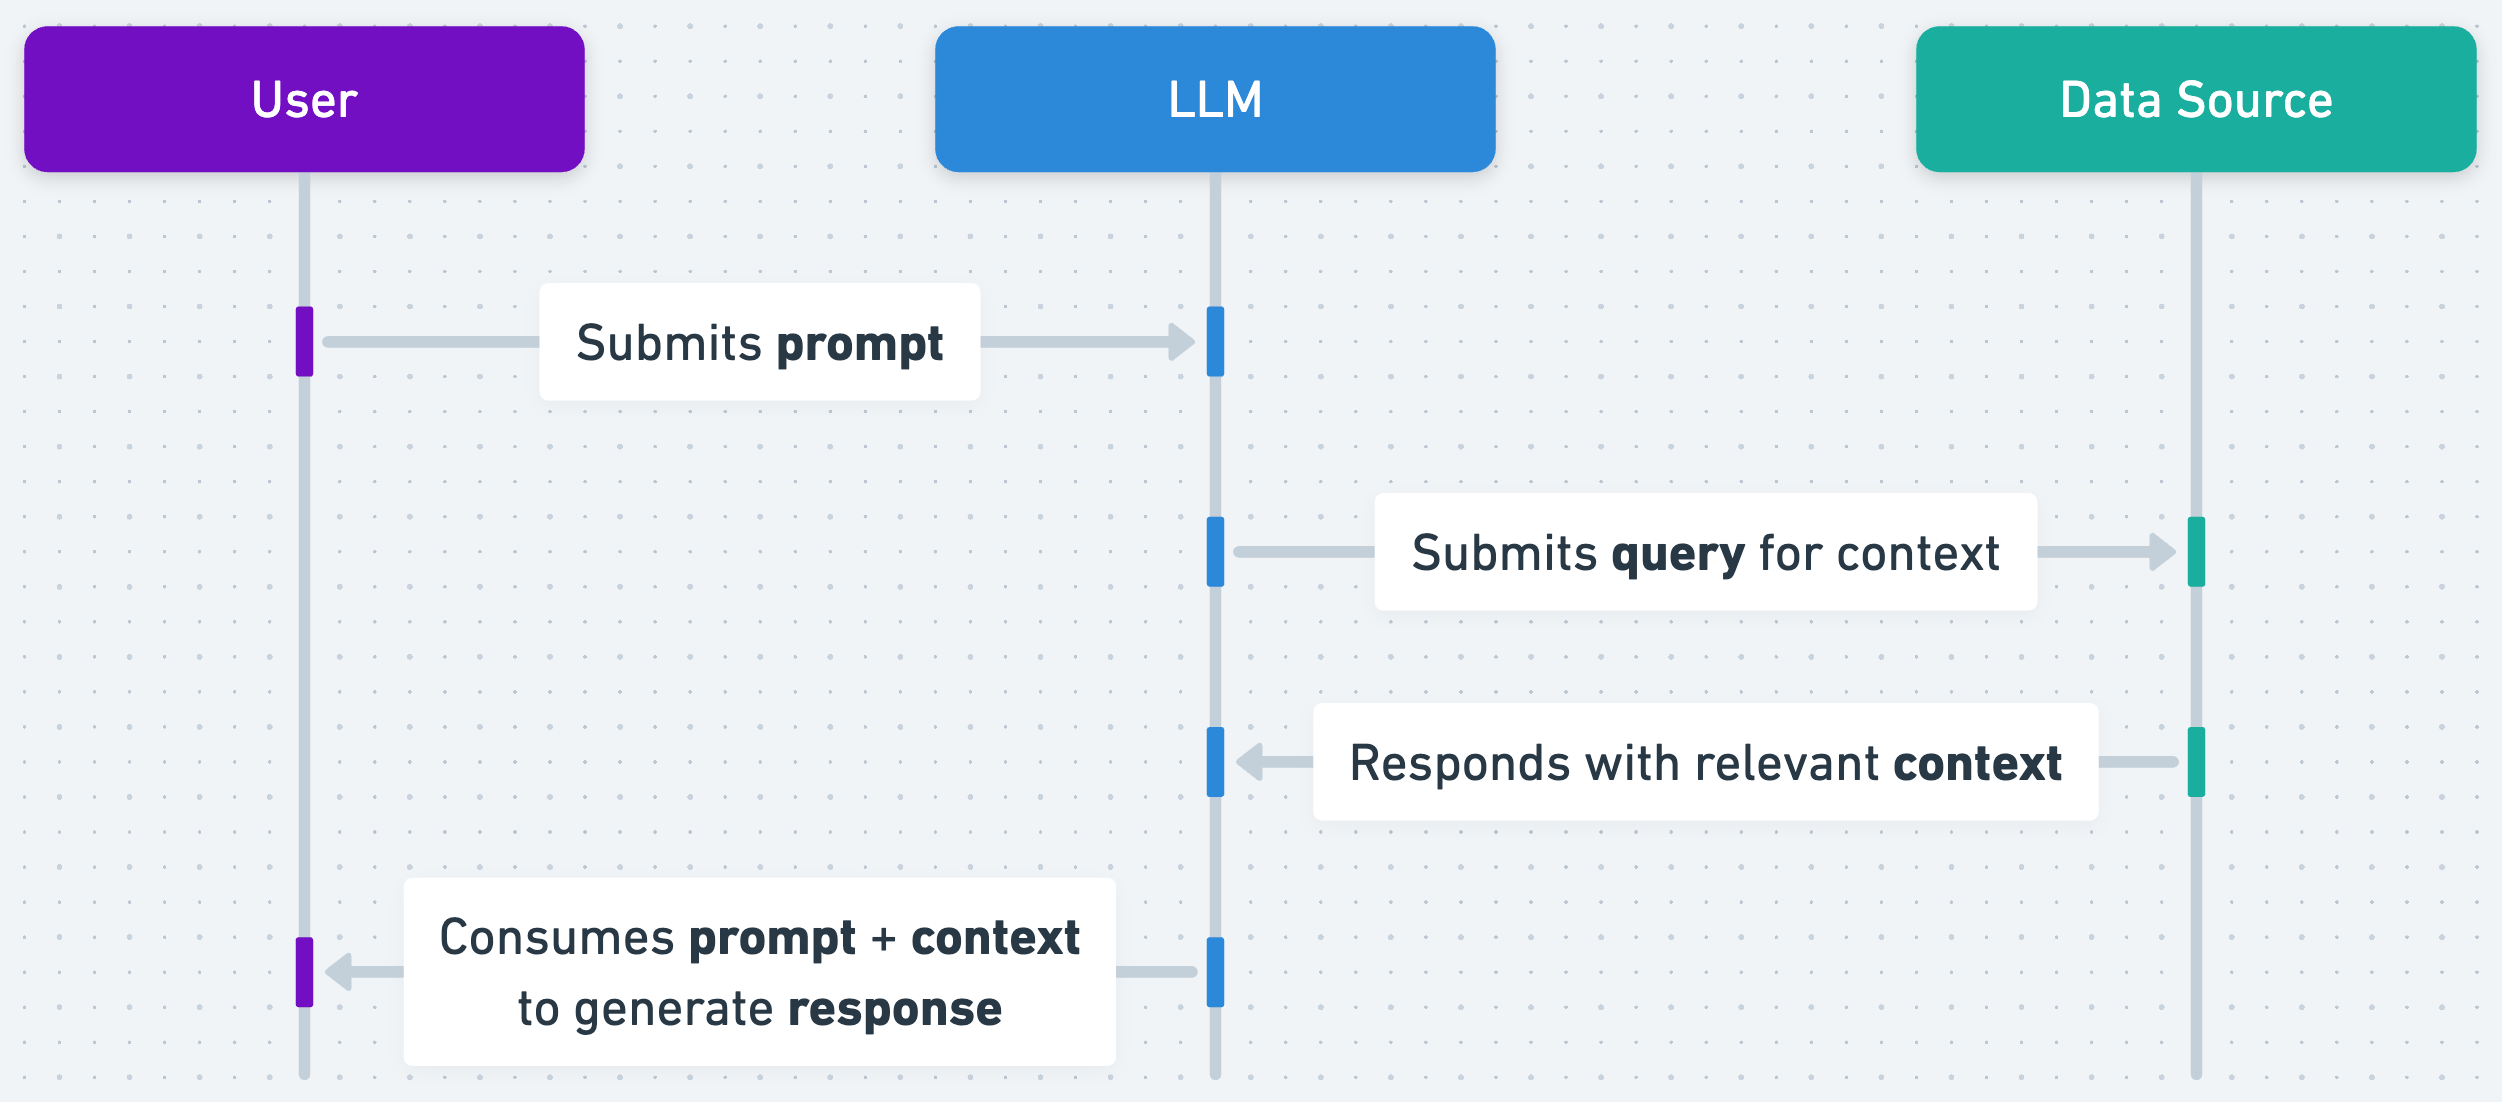
\includegraphics[width=.8\linewidth]{RAGProcess.png}
        \caption{A basic overview of a RAG workflow \autocite{openai_retrieval_nodate}.}
        \label{fig:RAGProcess}
    \end{figure}

    \textcite{siriwardhana_improving_2023} expanded upon the earlier works of \textcite{karpukhin_dense_2020} and \textcite{lewis_pre-training_2020} by creating 
    "RAG-end2end", which explored the capabilities of RAG on a dynamically updating knowledge store, meaning the LLM itself would not have to be retrained 
    every time the data updates, saving enormous amounts of processing power.
    
    RAG is dependent upon external knowledge stores such as vector databases, which store and process vectorised data
    for non-parametric memory \autocite{li_modernization_2023}, which makes them an essential part of the backend of 
    a RAG-enabled chatbot as studied by \textcite{odede_jaybot_2024}. 
    
    Many software options exist for
    vector databases, such as Milvus \autocite{wang_milvus_2021}, Pinecone \autocite{pinecone_pinecone_nodate} and Chroma\footnote{Also known as ChromaDB.} \autocite{chroma_chroma_nodate}.
    A study by \textcite{xie_brief_2023} compared these three, citing Pinecone's 'robust distributed computing capabilities and scalability', and its common usage 
    in real-time searching scenarios.
    
    Pinecone was also used in chatbots by \textcite{odede_jaybot_2024} and \textcite{singer_development_2024}, showcasing its potential as a vector database solution
    for chatbots.

    LangChain \autocite{langchain_introduction_nodate} is a popular open-source framework for RAG pipelines that can be used to connect backend elements 
    together, as described by \textcite{singer_development_2024} when they used it to chunk their text data and connect to their Pinecone vector database to store 
    the embedded data. 
    
    % Pinecone has a free option, though I'm not sure if this project could use it? Sounds like an Ethics Form problem.


    \subsection{Chatbots / Conversational Agents}
    % I was quite confident in this section given how short and direct it is. However, you've put too much about RAG in here.
    % You'll therefore need to find something else to write about here, perhaps things like Siri and Google Assistant?

    Conversational agents, better known as chatbots, leverage MLP in order to simulate a conversational flow 
    between a user and machine, and have become mainstream products in recent years \autocite{liao_all_2018},
    though have existed as far back as 1966 with the creation of "ELIZA" for the IBM-7094 \autocite{weizenbaum_elizacomputer_1966}.
    As time has passed, advancements in chatbots have occurred in "waves", where each new wave has brought a major innovation \autocite{schobel_charting_2024}.

    \begin{figure}[H] 
        \centering
        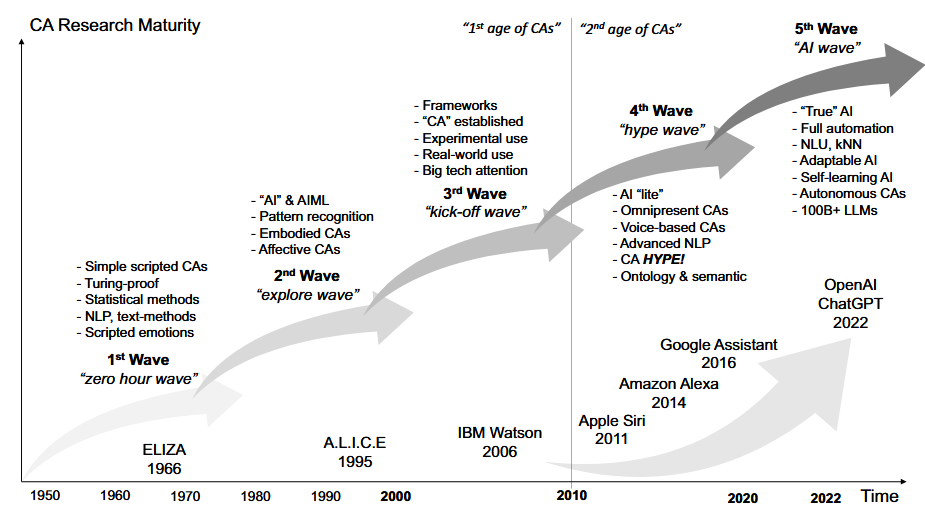
\includegraphics[width=.8\linewidth]{ChatbotWaves.png}
        \caption{The five waves of conversational agent research \autocite{schobel_charting_2024}.}
        \label{fig:ChatbotWaves}
    \end{figure}

    As a product of the considerable developments in the field, chatbots are now widely used 
    across industries such as education \autocite{kuhail_interacting_2023}. However, the use of the latest wave of chatbots based on LLMs,
    especially in educational settings, poses significant risks as studied by \textcite{neumann_llm-driven_2024}
    due to the risk of hallucinations being interpreted as absolute fact, although \textcite{shuster_retrieval_2021} 
    argued that this risk can be greatly reduced through introducing RAG to the backend LLM, which is further backed 
    by the RAG-based chatbot created by \textcite{ge_development_2023}, which they found to also give superior answers
    in their medical field of study to those of a general-purpose chatbot without RAG.  


    Many platforms exist to aid chatbot development, though they are typically aimed at users from non-IT backgrounds 
    \autocite{srivastava_desirable_2020}. Popular platforms include IBM's watsonx Assistant \autocite{ibm_ibm_2024},
    Google's Dialogflow \autocite{google_conversational_nodate} and Microsoft's Bot Framework \autocite{microsoft_microsoft_nodate}.
    However, these are primarily targeted at enterprise clients which is reflected in their pricing. Instead of using these,
    the chatbot can be manually developed using LangChain as its framework.

    

    \subsection{User experience and Human-Computer Interaction}
    % Debating the removal of this section.
    % Even if you don't delete it, I still think it's the weakest section of the review.

    The way people interact with their devices has drastically evolved over the years, from early MS-DOS command-line 
    interfaces (CLIs) to mouse-based graphical user interfaces (GUIs), to touch screens \autocite{kotian_systematic_2024}, greatly broadening
    the userbase of computers to a vast majority of the world's 
    population. Therefore, inclusive and accessible design is increasingly important to maximise the audience of any software,
    especially considering the growing disabled population \autocite{putnam_how_2012}. 
    
    As well as being inclusive, the design 
    should also be user-centred, meaning it should be an iterative process that is constantly taking user feedback 
    into account \autocite{chammas_closer_2015}. However, there are some barriers in this process when developing 
    chatbots, as studied by \textcite{clark_what_2019} in their survey of university students who stated that they would 
    always view a chatbot as a tool, and would not converse with them in the same way as they would a person, which would 
    limit their potential use and hinder the overall design process. 

    In this same context, it is also important to understand that users may struggle
    to get the chatbot to respond with information they want, as their prompts may be poorly understood
    due to issues like overgeneralisation \autocite{zamfirescu-pereira_why_2023}, and that users can quickly 
    grow impatient after around 2 to 6 failed attempts, often branding the product as poor if this occurs \autocite{luger_like_2016}.


    \pagebreak 

    \section{Summary}
    % I still think this is quite poor, but I don't know what else to say?

    In conclusion, this literature review has revealed multiple key areas of focus for the development of the 
    chatbot. The overall design of the chatbot must be iterative and human-centred, and user feedback should 
    be obtained at every possible opportunity to ensure the resultant product is high quality. A deep exploration 
    into AI, specifically in its applications in NLP and LLMs, has revealed that the best option for the chatbot 
    will be to leverage a pre-existing cloud-based LLM's RAG capabilities, as to do so on a local machine would require an infeasible amount of processing power.
    The non-parametric memory accessed through RAG would be a vector database created with Pinecone storing embeddings generated by OpenAI's text-embeddings-3-small 
    model, and the overall framework will be LangChain. This will keep the cost of the project low while maintaining a tolerable level of quality in the bot's responses.

    % Additionally, the discovery of many issues in the development of chatbots will greatly influence the design 
    % process, such as the need for users to be able to access the information they want in as few queries as 
    % possible to ensure user retention. Doing so will require prompt engineering to ensure that the LLM backend 
    % is generating specific information via RAG to ensure it is not giving irrelevant information.


    \begin{landscape}

    \chapter{Appendix}

    \section{Gantt Chart}

    \begin{figure}[H]
        \centering
        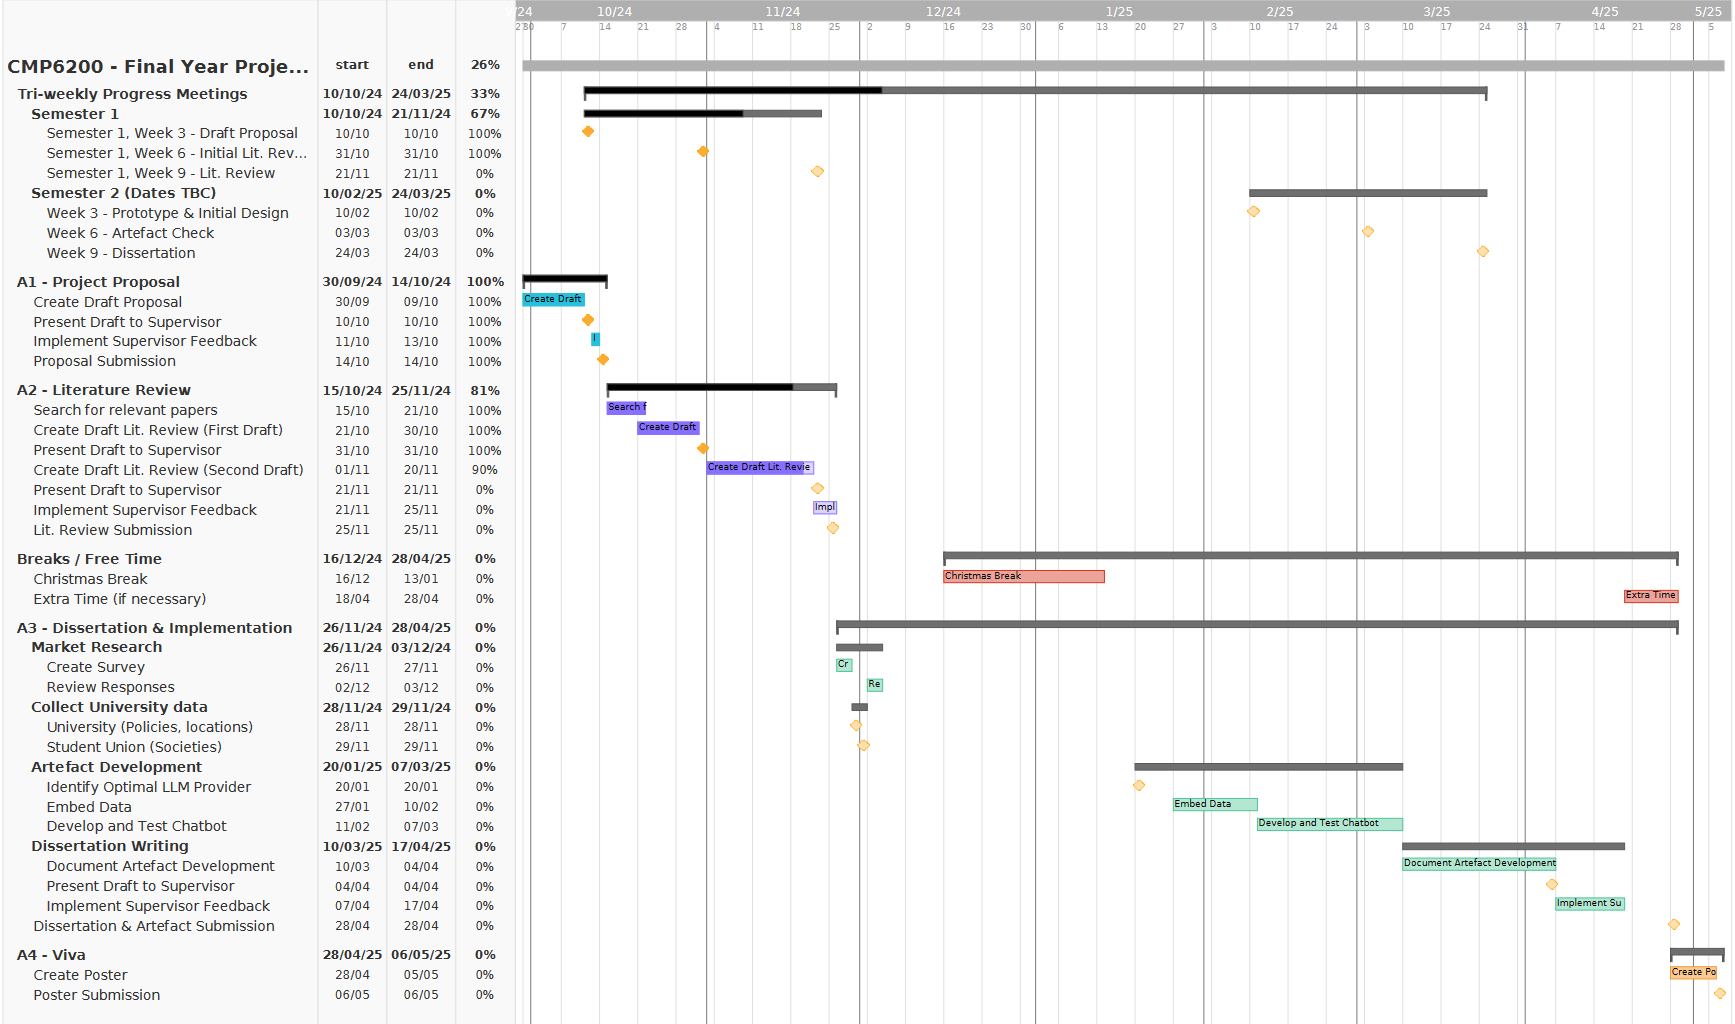
\includegraphics[width=.9\linewidth]{LitReviewGantt.png}
        \caption{The updated Gantt Chart for the development timeline.}
        \label{fig:gantt}
    \end{figure}

    \end{landscape}

    \printbibliography[keyword={refs}, title = {References}]
    \addcontentsline{toc}{chapter}{References}

    % Invisible citing bib sources so that they'll appear in the bibliography, as they won't show up unless cited.
    \nocite{IBMAIDef}
    \nocite{ICOAIDef}
    \nocite{IBMGenAI}
    \nocite{MITGenAI}
    \nocite{CloudflareLLM}
    \nocite{IBMNLP}
    \nocite{aws_what_nodate}
    \nocite{databricks_retrieval_2023}
    \nocite{elastic_what_nodate}
    \nocite{confident_ai_llm_nodate}

    \printbibliography[keyword={bib}, title = {Bibliography~~~~~~~~~~~~\small{Sources consulted but not directly cited}}]
    \addcontentsline{toc}{chapter}{Bibliography}

\end{document}